\chapter{減衰通信路を用いた通信}
減衰通信路を用いた通信を行う場合の通信容量を計算する。
以下は通信容量のグラフを書くためのプログラムである。

\begin{lstlisting}[caption=減衰通信路の通信容量,label=program5_1]
import japanize_matplotlib
x=np.arange(0,5,0.01)
y1=[]
arate=0.05 #@param {type: "number"}
for x_val in x:
  q_state=Qstate(x_val)
  q_state.attenuate(arate)
  p=norm.cdf(0,loc=q_state.alpha,scale=np.sqrt(q_state.a[0][0]))
  c=1+p*np.log(p)+(1-p)*np.log(1-p)
  y1.append(c)
y2=[]
for x_val in x:
  q_state=Qstate(x_val)
  q_state.attenuate(np.sqrt(arate))
  q_state.amplificate(1/np.sqrt(arate))
  q_state.attenuate(np.sqrt(arate))
  p=norm.cdf(0,loc=q_state.alpha,scale=np.sqrt(q_state.a[0][0]))
  c=1+p*np.log(p)+(1-p)*np.log(1-p)
  y2.append(c)

plt.plot(x,y1,label="増幅器なし",c="black",ls="dotted")
plt.plot(x,y2,label="増幅器あり",c="black",ls="-")
plt.legend()
plt.show()
\end{lstlisting}

\figref{Fig5_1}は、透過率$\lambda=0.05$の時の通信容量のグラフを表している。実線は増幅器ありの場合、点線は増幅器なしの場合のグラフである。グラフの横軸は信号の振幅値を表し、縦軸は通信容量を表している。グラフより、透過率$\lambda=0.05$の場合は、増幅器を設置することにより、通信容量を大きくする効果があることがわかる。

    \begin{figure}[H]
        \centering   
        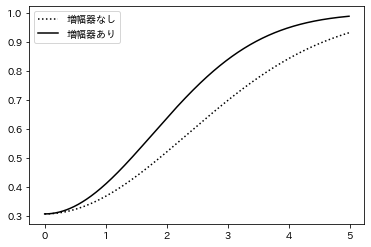
\includegraphics[width=1\textwidth]{img/Fig5_1.png}
        \caption[sample image (png)]{$\lambda=0.05$のときの通信容量の変化}
        \label{Fig5_1}
    \end{figure}

\newpage
\figref{Fig5_2}は、透過率$\lambda=0.1$の時の通信容量のグラフを表している。実線は増幅器ありの場合、点線は増幅器なしの場合のグラフである。グラフの横軸は信号の振幅値を表し、縦軸は通信容量を表している。グラフより、透過率$\lambda=0.1$の場合は、増幅器を設置することにより、通信容量は大きいが、$\lambda=0.05$の時よりほどではないことがわかる。

    \begin{figure}[H]
        \centering   
        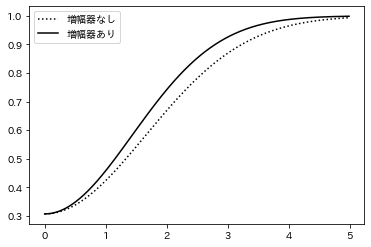
\includegraphics[width=1\textwidth]{img/Fig5_2.png}
        \caption[sample image (png)]{$\lambda=0.1$のときの通信容量の変化}
        \label{Fig5_2}
    \end{figure}


\newpage
\figref{Fig5_3}は、透過率$\lambda=0.2$の時の通信容量のグラフを表している。実線は増幅器ありの場合、点線は増幅器なしの場合のグラフである。グラフの横軸は信号の振幅値を表し、縦軸は通信容量を表している。グラフより、透過率$\lambda=0.2$の場合は、増幅器を設置していても通信容量はほぼ変わらないことがわかる。

    \begin{figure}[H]
        \centering   
        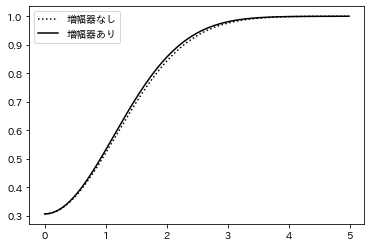
\includegraphics[width=1\textwidth]{img/Fig5_3.png}
        \caption[sample image (png)]{$\lambda=0.2$のときの通信容量の変化}
        \label{Fig5_3}
    \end{figure}


\newpage
\figref{Fig5_4}は、透過率$\lambda=0.3$の時の通信容量のグラフを表している。実線は増幅器ありの場合、点線は増幅器なしの場合のグラフである。グラフの横軸は信号の振幅値を表し、縦軸は通信容量を表している。グラフより、透過率$\lambda=0.3$の場合も増幅器を設置していても通信容量はほぼ変わらないことがわかる。

    \begin{figure}[H]
        \centering   
        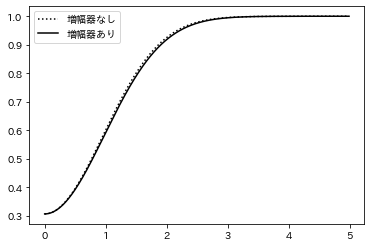
\includegraphics[width=1\textwidth]{img/Fig5_4.png}
        \caption[sample image (png)]{$\lambda=0.3$のときの通信容量の変化}
        \label{Fig5_4}
    \end{figure}

\newpage
\figref{Fig5_5}は、透過率$\lambda=0.6$の時の通信容量のグラフを表している。実線は増幅器ありの場合、点線は増幅器なしの場合のグラフである。グラフの横軸は信号の振幅値を表し、縦軸は通信容量を表している。グラフより、透過率$\lambda=0.6$の場合も増幅器を設置していても通信容量はほぼ変わらないことがわかる。

    \begin{figure}[H]
        \centering   
        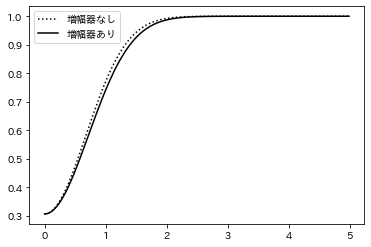
\includegraphics[width=1\textwidth]{img/Fig5_5.png}
        \caption[sample image (png)]{$\lambda=0.6$のときの通信容量の変化}
        \label{Fig5_5}
    \end{figure}


\newpage
\figref{Fig5_6}は、透過率$\lambda=0.9$の時の通信容量のグラフを表している。実線は増幅器ありの場合、点線は増幅器なしの場合のグラフである。グラフの横軸は信号の振幅値を表し、縦軸は通信容量を表している。グラフより、透過率$\lambda=0.9$の場合も増幅器を設置していても通信容量はほぼ変わらないことがわかる。

    \begin{figure}[H]
        \centering   
        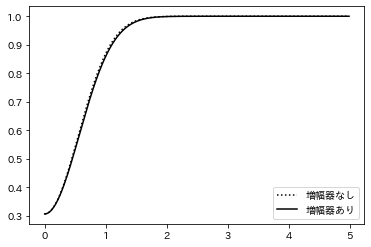
\includegraphics[width=1\textwidth]{img/Fig5_6.png}
        \caption[sample image (png)]{$\lambda=0.9$のときの通信容量の変化}
        \label{Fig5_6}
    \end{figure}






    
